\section{Explaining the Role of Symbols} \label{sec:empirical-studies-explaining-the-role-of-symbols}

In the previous set of experiments we showed that our theory holds given that the models trained with the aid of symbols outperformed the models that were trained in the absence of symbols. We also showed that there was not much difference in the effectiveness of both the explicit and implicit forms of providing symbols. The next set of experiments investigate the second objective of our research which is to establish the reason why symbols improve learning in artificial neural networks. We start with an experiment that attempts to show that symbols help the artificial learner discover a general solution to the problem, similar to how they are used by humans. Based on the results, we explain the role that symbols play in the learning process.

\subsection{Experiment 4: Recurrent Neural Network's Ability to Discover an Algorithm for Arithmetic Operations} \label{sec:experiment-4}

\subsubsection{Objective}

In Section \ref{sec:theory-approach-methodology-pattern-matching-vs-learning-an-algorithm} we described two possible methods a neural network can learn to perform these arithmetic operations, either by (1) memorizing the input patterns along with the corresponding output, effectively doing pattern matching, or (2) by learning an algorithm that is able to generalize to patterns that the model has not seen before. In the prior experiments, we have shown the former to be true. However, we wish to show that with the aid of appropriate symbols a recurrent neural network is capable of discovering a representation of an algorithm that performs the corresponding mathematical operation.

In this experiment, we attempt to understand whether or not recurrent neural networks are able to accomplish that goal. To verify if that is indeed the case, we train our models on a subset of the combinations of digits. The remaining set of combinations are used to test the trained models. If the models perform well on this unseen set of combinations, this would show that the recurrent neural networks are able to generalize to unseen combinations of digits and is therefore proof that the machine learning system has discovered an algorithm for the arithmetic operations. Otherwise the models trained in the previous experiments are simply doing pattern matching.

\subsubsection{Method}

We develop and train five models for this experiment to perform all four arithmetic operations on the MNIST dataset of handwritten digits. Similar to how the models in Experiment 3 in Section \ref{sec:experiment-3} were trained,  the first model is trained with 0\% symbols, the second with 25\% symbols present, the third with 50\% symbols present, the fourth with 75\% symbols present and finally the fifth with 100\% symbols. All five models have the same architecture that accepts a sequence of three 28x28 images. The first two images are of the handwritten digits representing the operands of the operation. The third image is that of the operator. The models output two one-hot vectors. For the first two time steps the output is the one-hot vector representation of the input digits. On the third step the output is a one-hot vector representation of the result of the operation. Two hidden layers are used each with 512 LSTM units.

The five datasets used in Experiment 3 are also used for this experiment. The difference is that not all combinations of digits are used for training. For each of the five datasets, a subset composed of 80\% of the digit combinations are selected for training for each of the four operators, making sure that each unique digit would be present at least once on either side of the arithmetic operator. We call this the ``seen" dataset since the models are exposed to these combinations during training. The remaining 20\% combinations are the ``unseen" test set that we use to determine if the models are able to generalize to unseen operations and therefore are able to learn an algorithm. The samples in the seen training set are distributed into training, validation and test sets using k-fold cross-validation where k is set to 5. All the samples in the unseen test set are used for testing after the models are trained on the seen dataset. The networks are trained using the Adam optimizer with the mean square error as the loss function and a learning rate of 0.001. Training is performed over 200 epochs in batches of 100 and the model performing best on the validation set is saved and used for testing.

\subsubsection{Results}

\begin{table}[p!]
	\center
	\caption{A comparison of the mean accuracy and standard deviation along with the p-value of a hypothesis t-Test when compared to the 0\% symbols model when tested on the test set of \textbf{seen} combinations.}
	\label{tab:experiment-4-results-table-seen}
	\begin{tabular}{ |c|c|c|c| } 
		\hline
		\% Symbols Present & Accuracy (\%) & Standard Deviation  & p-value\\ 
		0\% & 40.68 & 0.0420 & NA \\  
		25\% & 57.48 & 0.0211 & 0.00383\\  
		50\% & 61.38 & 0.0504 & 0.0 \\  
		75\% & 69.44 & 0.0136 & 0.0\\  
		100\% & 78.23 & 0.0134 & 0.0\\  
		\hline
	\end{tabular}
\end{table}

\begin{table}[p!]
	\center
	\caption{A comparison of the mean accuracy and standard deviation along with the p-value of a hypothesis t-Test when compared to the 0\% symbols model when tested on the test set of \textbf{unseen} combinations.}
	\label{tab:experiment-4-results-table-unseen}
	\begin{tabular}{ |c|c|c|c| } 
		\hline
		\% Symbol Presence & Accuracy (\%) & Standard Deviation  & p-value\\ 
		0\% & 1.00 & 0.0 & NA \\  
		25\% & 3.00 & 0.0240 & 0.374\\  
		50\% & 4.00 & 0.0367 & 0.208 \\  
		75\% & 2.00 & 0.0240 & 0.621\\  
		100\% & 3.00 & 0.0392 & 0.477\\  
		\hline
	\end{tabular}
\end{table}

\begin{figure}[p!]%
	\centering
	\subfloat[Seen Test Combinations]{{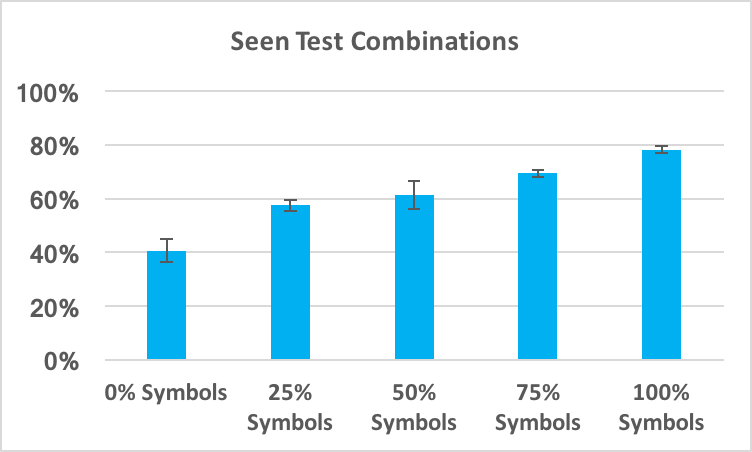
\includegraphics[width=0.5\textwidth]{experiment-4-results-chart-seen}}}%
	\subfloat[Unseen Test Combinations]{{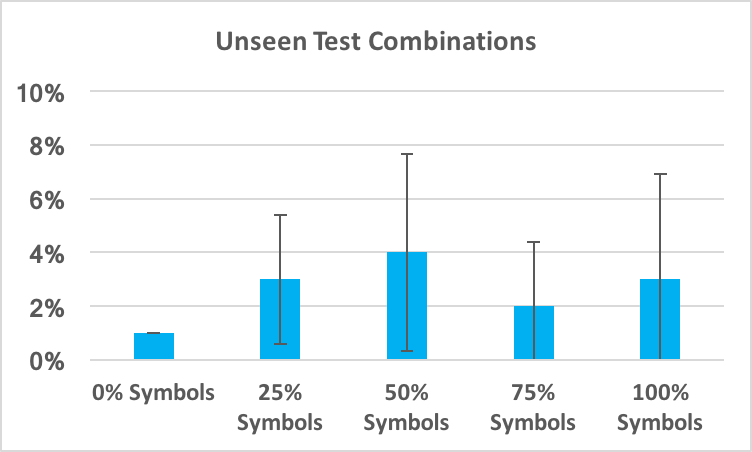
\includegraphics[width=0.5\textwidth]{experiment-4-results-chart-unseen}}}%
	\caption{A comparison of the mean accuracy and 95\% confidence intervals for each of the models when tested on both the \textbf{seen} and \textbf{unseen} test combinations.}
	\label{fig:experiment-4-results-chart}
\end{figure}

Table \ref{tab:experiment-4-results-table-seen} shows the mean accuracy, standard deviation and t-test p-value scores for the test set which uses the same operand combinations that the models were trained on. Table \ref{tab:experiment-4-results-table-unseen} shows these same metrics when the same models are tested on operand combinations they have never seen before. Figure \ref{fig:experiment-4-results-chart} shows graphs of these results along with 95\% confidence intervals.

Table \ref{tab:experiment-4-results-table-seen} shows similar accuracies to those obtained in Experiment 2 with the models trained in the presence of symbols outperforming the ones trained without symbols. However, the models when tested on the unseen dataset show poor performance regardless of whether they are trained with symbols or not.

\subsubsection{Discussion}

It is clear from these results that the current recurrent neural network models are unable to generalize to unseen combinations of operands. They are unable to discover a representation for an algorithm for the arithmetic operations. The models perform well on the previously experienced combinations by developing a sequential mapping function for those seen operand combinations.

In the next section, we describe an experiment that examines our theory in Section \ref{sec:theory-approach-methodology-pattern-matching-vs-learning-an-algorithm} to understand how this pattern matching works and how the presence of symbols makes this process more effective. Later, we present a different approach that uses a modified representation of the symbols as discussed in Section \ref{sec:theory-approach-methodology-temperature-encoding}. Using this new representation, we are able to develop a model that performs well on unseen test sets.

\subsection{Experiment 5: Using Symbols Only to Learn Arithmetic Operations} \label{sec:experiment-5}

\subsubsection{Objective}

We have shown that the presence of symbols improves the accuracy of learning with a limited dataset of noisy examples. In Experiment 3 in Section \ref{sec:experiment-3}, we showed that this was due to the effectiveness of symbols at learning a mapping function. In the previous experiment however, we have failed to show that symbols allow neural networks to go beyond learning mapping functions and actually discover an algorithm to perform the arithmetic operations. In this experiment, we constrain and simplify the problem to make it easier for the models we are developing to reach the desired objective of learning an algorithm. We will train recurrent neural networks to perform addition using the symbolic features alone without introducing the MNIST handwritten digits. The goal here is the same as that of Experiment 4 in Section \ref{sec:experiment-4} where we want to force the network to generalize to unseen combinations of digits.

Besides constraining the input features, we also take a different approach to analyzing the behavior of the trained recurrent neural networks, by visualizing the outputs of the hidden layers of the models using a concept know as activations clustering. With activations clustering, the output value of each unit in the hidden recurrent layers ($h_t$) is mapped to a pixel intensity where an output of -1 would map to 0 and an output of 1 would map to 255. Each unit would be assigned a region on an image and that region would be filled using the pixel intensity assigned when a digit is presented to the trained model on each time step. Figure \ref{fig:activations-cluster-explained} shows an example of an activations cluster. The activations clusters should allow us to confirm that the presence of symbols allows for more consistency in the representation which leads to the improved accuracy. The clusters may also shed some insight into why the networks fail to develop an algorithm.

We will also add an additional time step to the recurrent sequence. Like before, the first time step is the right hand operand, the second time step is the left hand operand, the third time step is the operator which now only outputs the least significant digit of the result. The additional fourth time step is an equals sign which signifies to the model to output the most significant digit of the result. This change was made so that we can determine if there is any relationship between what is being output on the least significant one-hot vector and the most significant one. This also resembles how we as humans do addition. We consume one input digit at a time and we produce one output digit at a time, making note of carry forward digits, if necessary.


\subsubsection{Method}

\begin{figure}
	\centering
	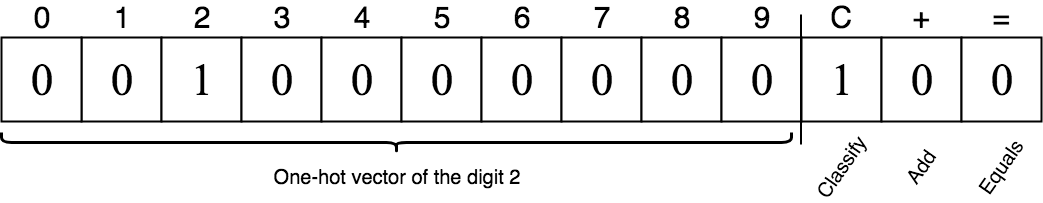
\includegraphics[max width=\textwidth]{experiment-5-input}
	\caption{An example of an input vector for the digit 2 on the first time step. The first ten features are for the one-hot symbol. The 11th (C) feature when set, feature instructs the RNN to output the class at that time step. The 12th (+) feature when set, instructs the network to output the least significant digit of the result. The 13th (=) feature when set, instructs the RNN to output the most significant digit of the result.}
	\label{fig:experiment-5-input}
\end{figure}

The models developed for this experiment accept a sequence of four vectors, each vector is composed of thirteen elements. Figure \ref{fig:experiment-5-input} depicts the structure of the input vectors. The first ten elements represent the one-hot vector. Element 11 is set to one when we want the network to perform classification and output a one-hot vector representing the input operand, zero otherwise. This is always set to one when the operands are presented to the network to signify to the network that an input symbol is being presented on the intermediate time steps. Element 12 is set to one at the third time step. This element indicates that the addition should be performed and that the least significant digit of the output should be produced. The element is set to zero otherwise. Finally, element 13 is set to one on the fourth time step when the most significant digit of the result of the addition is presented on the output.

\begin{figure}
	\centering
	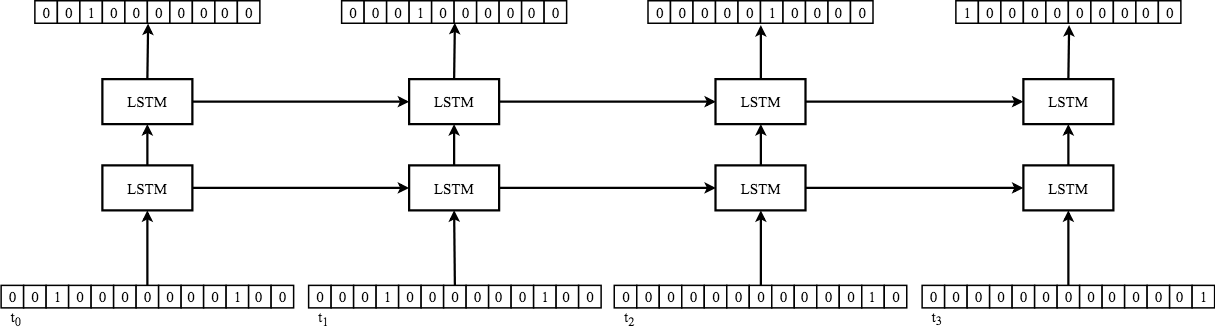
\includegraphics[max width=\textwidth]{experiment-6-architecture}
	\caption{The constrained symbol only architecture learning to perform 2 + 3.}
	\label{fig:experiment-6-architecture}
\end{figure}

The output layer of the models consists of 10 elements representing a one-hot vector output. When the first operand is presented on the input layer, the network outputs the same digit on the output layer. The same goes for the second operand on the second time step. When an input that has the 12th element set to one is presented on the third time step, the network outputs the least significant digit of the result of adding the operands together. Finally, on the fourth time step when an input having the 13th element set to one is presented to the model, the model outputs the most significant digit of the addition. Figure \ref{fig:experiment-6-architecture} depicts how the input and output layers interact on each time step.

A total of four recurrent neural network architectures were developed using the same input and output layer structures presented above. The models vary in the number and size of the recurrent hidden layers.  The following lists the composition of the hidden layers for each of the four models developed:
\begin{itemize}
	\item \textbf{Model A}: One hidden layer with 10 LSTM units each.
	\item \textbf{Model B}: Two hidden layers with 10 LSTM units each.
	\item \textbf{Model C}: Three hidden layers with 10 LSTM units each.
	\item \textbf{Model D}: Two hidden layers with 20 LSTM units each.
\end{itemize}

The dataset is composed by forming all possible 100 combinations of operands. A subset of 80 combinations are selected for training from that dataset, making sure that each unique digit would be present at least once on either side of the addition operator. That same training set is also used for validation and as the test set of seen combinations. The remaining 20 combinations are used as the unseen combinations test set. Each model is trained and tested five times and the mean accuracy of each model is recorded when applying both the seen test set and the unseen test set on the trained model. Training is performed over 5000 epochs in batches of 10 using the Adam optimizer algorithm and the mean square error loss function with a learning rate of 0.001.

\subsubsection{Results}

\begin{figure}
	\centering
	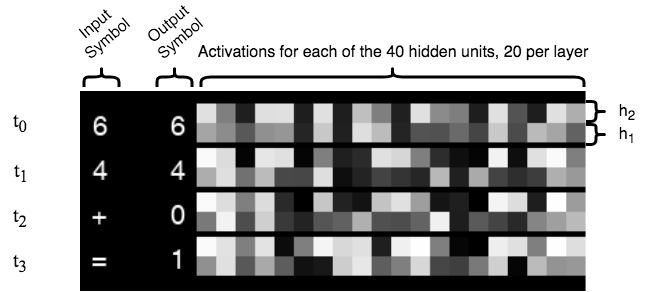
\includegraphics[max width=\textwidth]{activations-cluster-explained}
	\caption{An activations cluster generated when presenting the one-hot symbols of the operation 6 + 4 to the trained Model D. The symbols are displayed in this image as digits for clarity.}
	\label{fig:activations-cluster-explained}
\end{figure}

Table \ref{tab:experiment-6-results-table} shows the mean accuracies for each of the architectures developed. The table shows these values for both the full training set and the unseen test set. Figures \ref{fig:activations-cluster-explained} and \ref{fig:activations-cluster-carry} show some of the activations clusters that are produced when applying the seen dataset to Model D (the best performing model).

Figure \ref{fig:activations-cluster-explained} shows the result of rendering the activations cluster when applying the operand sequence of 6 + 4 to the trained Model D. The figure shows four rows of items, each row represents a single time step. For each time step, the figure depicts the input to the network, the output the network produces and the activations on the hidden units. The inputs and outputs are rendered in the figure as digits for clarity. Forty activations are shown for each time step, one for each hidden unit. The activations are split into two rows, each row holds the activations for one of the two hidden layers.

\begin{table}[h]
	\center
	\caption{A comparison of the mean accuracy of each of the four models developed when tested on the test set of \textbf{seen} combinations as well as the test set of \textbf{unseen} combinations.}
	\label{tab:experiment-6-results-table}
	\begin{tabular}{ |c|c|c| } 
		\hline
		Model & Accuracy - Seen (\%) & Accuracy - Unseen (\%)\\ 
		Model A & 75.0 & 5.0\\  
		Model B & 75.0 & 5.0\\  
		Model C & 75.0 & 5.0\\  
		Model D & 100.0 & 5.0\\
		\hline
	\end{tabular}
\end{table}

\subsubsection{Discussion}

It is clear from the results that even when constraining the model to only use one-hot symbols as inputs, the recurrent networks fail to generalize to the unseen dataset, even though they perform very well on the seen dataset. This shows that even when using clear one-hot symbols the neural network is still not able to discover a set of weights that can represent an algorithm that performs the addition operation.

\begin{figure}
	\centering
	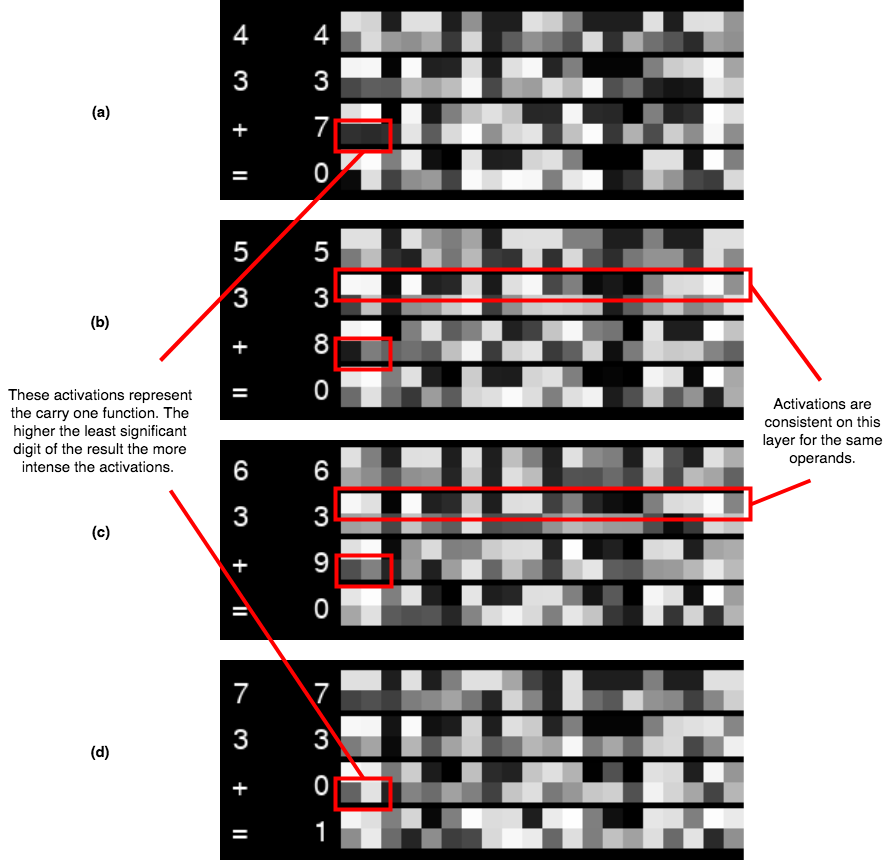
\includegraphics[max width=\textwidth]{activations-cluster-carry-annotated}
	\caption{A series of activations from Model D showing how the intensity in the bottom left region of the third time step changes when the output transitions from 7 through 8 and 9 to 10.}%
	\label{fig:activations-cluster-carry}%
\end{figure}

When analyzing the sequence of activations clusters in Figure \ref{fig:activations-cluster-carry}, we notice that the activations on the top layer ($h_2$) on any of the first two time steps are always consistent when the same operands are presented as exhibited by the digit 3 on the second time step of Figures \ref{fig:activations-cluster-carry} (a) to \ref{fig:activations-cluster-carry} (d). Also, the least and most significant digit outputs always have consistent activations on the top layer for the same results (see the fourth time step in Figures \ref{fig:activations-cluster-carry} (a), \ref{fig:activations-cluster-carry} (b) and \ref{fig:activations-cluster-carry} (c) and the third time step in Figure \ref{fig:activations-cluster-carry} (d)). By ``consistent" we mean that the same hidden units are producing the same intensities. These observations are in-line with the findings of Experiment 3 in Section \ref{sec:experiment-3} which shows that when successfully classifying the input digits, the recurrent neural networks discover a consistent internal representation that facilitates the execution of the arithmetic operations.

Another interesting pattern can be observed when analyzing the transition from the least significant digit time step to the most significant digit time step (see Figure \ref{fig:activations-cluster-carry}). The two most left-hand activations on the lower layer of the third (least significant digit) time step tend to be dark (indicating lower activations) when the least significant digit of the result is closer to zero than nine. The higher that digit the lighter the activations become. The variation in activations indicates that there is a signal being carried over from the least significant digit time step to the most significant digit time step. That signal forces the most significant output to flip from a zero to a one. When comparing this behavior with how we as humans perform addition, this process resembles the carry-one approach when writing out arithmetic problems with pen and paper. This shows that though for the most part the networks are still learning a mapping function, there are still some elements of an algorithm being developed within the network.

When further analyzing how humans learn to perform addition, we tend to convert the numbers into concepts that can be counted. More specifically with children, we represent numbers as collections of objects. So, 5 + 3 for example will be translated to a child as counting five ``apples" and counting another three ``apples" on top of the initial five. The symbols are able to represent quantity and ordinal relationships. One-hot vectors on the other hand don't capture these concepts; they are able to represent classes of digits which is why they assist in the development of good classifiers, but fail to develop models that can generally perform arithmetic. In the next set of experiments we use a different encoding for our symbols that better captures the ordinal nature of the digits.